% This file was adapted from ICLR2022_conference.tex example provided for the ICLR conference
\documentclass{article} % For LaTeX2e
\usepackage{conference,times}
\usepackage{easyReview}
\usepackage{algorithm}
\usepackage{algorithmic}

% Optional math commands from https://github.com/goodfeli/dlbook_notation.
\input{math_commands.tex}

\usepackage{amsthm,amssymb}

\newtheorem{theorem}{Theorem}[section]
\newtheorem{corollary}[theorem]{Corollary}
\newtheorem{lemma}[theorem]{Lemma}
\newtheorem{definition}[theorem]{Definition}

% Please leave these options as they are
\usepackage{hyperref}
\hypersetup{
    colorlinks=true,
    linkcolor=red,
    filecolor=magenta,
    urlcolor=blue,
    citecolor=purple,
    pdftitle={Glucose-Responsive Insulin Design via Hybrid Machine Learning, Molecular Dynamics, and Pareto Selection},
    pdfpagemode=FullScreen,
    }



\title{Glucose-Responsive Insulin Design via Hybrid Machine Learning, Molecular Dynamics, and Pareto Selection}

\author{Marius-Constantin Dinu \\
Independent Research \\
Computational Biology \\
\texttt{correspondence available upon request}}

\begin{document}


\maketitle

\begin{abstract}
Type 1 diabetes management remains constrained by insulin therapies that are dosed externally and therefore cannot adapt in real time to changing glycemic states. This gap motivates glucose-responsive insulin design, where molecular activity is attenuated in hypoglycemia and amplified in hyperglycemia. We study this objective as a computational prioritization problem rather than a full clinical development program: given insulin-centered molecular candidates, predict a state-conditional activity profile and select a shortlist for downstream experiments under bounded compute. The proposed method is a three-stage hybrid pipeline: a tri-state ranker enforces monotone low/normal/high behavior with uncertainty penalties; a mechanistic reranker augments machine-learning scores with paired-context molecular dynamics descriptors and explicit low-glucose safety gating; and an uncertainty-aware Pareto selector balances efficacy, hypoglycemia risk, and manufacturability. We provide formal definitions of objectives, feasible sets, and optimality criteria, and include theorem-level results with complete proofs for ordering and dominance properties. Validation uses a reproducible synthetic proxy protocol with fixed seeds, sweeps, confidence intervals, and symbolic checks. Relative to strong baselines, the selected pipeline improves tri-state rank correlation, reduces top-k false positives under safety constraints, raises nondominated shortlist quality, and passes symbolic assumption checks. The findings support a practical thesis: hybrid statistical-mechanistic ranking with explicit multi-objective uncertainty control can materially improve preclinical computational triage for glucose-responsive insulin candidates, while still exposing key data and translation gaps that must be addressed for broader external validity.
\end{abstract}

\section{Introduction}
Insulin replacement remains lifesaving in type 1 diabetes, yet externally administered insulin fundamentally lacks endogenous feedback. As a result, treatment remains exposed to the classical safety-control dilemma: aggressive dosing improves hyperglycemia but increases hypoglycemia risk, while conservative dosing lowers severe lows at the cost of chronic highs and broader metabolic burden. The glucose-responsive insulin literature has pursued an alternative principle for more than a decade, namely embedding glycemic feedback directly in molecular or material behavior so that effective activity increases when glucose is high and decreases when glucose is low \citep{src01,src02,src09,src10,src11}. Recent preclinical results have strengthened feasibility claims for both molecule-intrinsic and material-assisted designs \citep{src01,src12,src13,src41,src42,src43}. At the same time, translational uncertainty remains high because many candidate classes are evaluated with heterogeneous assays, and direct low/normal/high conditional benchmarks remain sparse \citep{src02,src10,src11,src44}.

These constraints naturally position computational filtering as an upstream decision layer. Instead of claiming full therapeutic optimization, we ask a narrower but practically consequential question: under fixed computational budget, can we select a shortlist of insulin-centered candidates that better respects conditional glycemic behavior and safety constraints than static affinity-centric pipelines? This framing matters beyond diabetes. Any therapeutic program that requires context-dependent activation, whether by metabolite levels, tissue microenvironment, or disease state, faces the same challenge of ranking under interacting efficacy, safety, and deployability objectives. Consequently, methods for robust conditional ranking in this domain are also relevant to broader adaptive biologics design.

The proposed pipeline is intentionally hybrid. Purely statistical rankers can scale but may overfit static surrogates and underestimate mechanism-linked failure modes. Purely mechanistic simulation can capture richer dynamics but is often too expensive for large candidate sets. We combine both with explicit uncertainty accounting and multi-objective selection constraints. The first stage enforces tri-state monotonic behavior during ranking. The second stage performs targeted mechanistic reranking on a computationally bounded shortlist. The third stage converts scalar ranking into constrained Pareto selection with uncertainty penalties. This structure is motivated by earlier evidence on glucose-responsive design chemistry \citep{src01,src03,src06,src15}, structure and interaction modeling \citep{src16,src17,src23,src33,src38}, and docking or affinity inference \citep{src24,src26,src27,src28,src39,src40}.

We contribute the following:
\begin{itemize}
\item We formulate glucose-responsive insulin prioritization as a tri-state constrained ranking problem with explicit objective, feasible set, and optimality criterion under bounded compute.
\item We introduce a hybrid reranking functional that couples machine-learning signal, paired-context molecular dynamics differentials, uncertainty penalties, and low-glucose safety gating.
\item We define an uncertainty-aware Pareto selection rule over efficacy, safety, and manufacturability proxies, and provide theorem-level properties for dominance pruning and robustness trade-off behavior.
\item We provide a reproducible evaluation protocol with fixed seeds, confidence intervals, symbolic consistency checks, and regime-stratified confirmatory diagnostics.
\end{itemize}

The remainder of the paper is organized as follows. \Secref{sec:related} situates the method against prior GRI and computational design literature. \Secref{sec:problem} defines symbols, assumptions, constraints, and objective criteria. \Secref{sec:method} presents the three-stage method, formal statements, and pseudocode. \Secref{sec:experiments} describes the validation protocol, while \secref{sec:results} reports quantitative and symbolic outcomes. \Secref{sec:limitations} discusses caveats and future experiments, and \secref{sec:conclusion} closes.

\section{Background and Related Work}
\label{sec:related}
\subsection{Glucose-Responsive Insulin Design Landscape}
The GRI landscape contains two broad families. The first is molecule-intrinsic modulation, where insulin analog chemistry or complexation directly changes receptor-accessible behavior across glycemic states \citep{src01,src12,src13,src41}. The second is material-mediated control, where polymers, vesicles, or transdermal systems modulate release rates through glucose-sensitive transport or reaction pathways \citep{src03,src04,src06,src42,src44}. Both families can be effective under specific conditions, but each carries known trade-offs. Molecule-centric strategies can offer direct pharmacological relevance, yet often demand precise tuning of affinity shifts and stability. Material-centric strategies provide rich control knobs but may face long-term biocompatibility, selectivity, or manufacturing constraints \citep{src09,src10,src11,src44}.

A recurring gap across studies is comparability. Metrics and assay conditions vary substantially, especially when reporting low-glucose safety margins versus high-glucose efficacy windows. This heterogeneity complicates direct ranking across candidate mechanisms and slows objective-setting for computational models. Our work does not claim to solve benchmark standardization, but it addresses the immediate practical consequence: when labels are sparse and noisy, ranking objectives must encode directional behavior and uncertainty more explicitly than standard static affinity scoring.

\subsection{Computational Modeling for Conditional Molecular Prioritization}
Recent structure-prediction and interaction-modeling advances materially improve candidate representation quality \citep{src16,src17,src23,src33,src38}. Generative design methods expand proposal space for sequence and scaffold hypotheses \citep{src18,src19}. Meanwhile, docking and affinity frameworks provide tractable screening signals \citep{src24,src26,src27,src28,src39,src40}. However, most such pipelines optimize static endpoints, for example pose quality or absolute affinity at one condition. For glucose-responsive insulin ranking, the key target is differential behavior across physiologic states, not merely high nominal affinity in a single context.

This distinction motivates two design decisions in our method. First, we optimize pairwise state differences and monotonic penalties directly instead of post hoc differencing independently trained predictors. Second, we add a mechanistic correction layer for top-ranked candidates because static predictors alone can mis-rank candidates with brittle state-dependent dynamics. The mechanistic layer is lightweight by design, aligned with the broader role of molecular dynamics as a focused validation signal in drug discovery when exhaustive simulation is infeasible \citep{src36}.

\subsection{Data Infrastructure, Uncertainty, and Multi-Objective Selection}
Public infrastructures such as PDBbind, BindingDB, UniProt, and RCSB PDB remain essential for pretraining, transfer, and annotation \citep{src29,src30,src31,src32,src37}. Yet none is purpose-built for paired low/normal/high glucose-response labels on engineered insulin candidates. This gap increases epistemic uncertainty and makes calibration central to trustworthy shortlist construction.

Finally, translational prioritization is inherently multi-objective. Candidate sets that maximize a single efficacy proxy often degrade safety or manufacturability constraints. Prior reviews repeatedly call for explicit co-optimization rather than serial thresholding \citep{src10,src11,src15}. Our Pareto stage operationalizes this recommendation with uncertainty-aware constrained selection, producing a shortlist that better preserves trade-off structure for downstream experimental triage.

\section{Problem Setting, Symbols, and Assumptions}
\label{sec:problem}
We consider a finite candidate set $\mathcal{C}$ of insulin-centered molecular designs. Each candidate $c \in \mathcal{C}$ has feature representation $\vx_c \in \mathbb{R}^d$ assembled from sequence, structure, and interaction descriptors. Glycemic state space is $\mathcal{G}=\{G_{\mathrm{low}},G_{\mathrm{norm}},G_{\mathrm{high}}\}$, corresponding to hypoglycemic, euglycemic, and hyperglycemic conditions. A state-conditional activity predictor $A_{\vtheta}(c,G)$ estimates receptor-relevant activity for candidate $c$ at state $G$, and $u(c)\ge 0$ denotes predictive uncertainty.

The decision problem is not unconstrained maximization. It is constrained shortlist construction under compute, safety, and uncertainty requirements. Let $K$ be final shortlist size and $B$ be total computational budget. We seek a policy that maximizes conditional efficacy while satisfying low-glucose safety and tractability constraints. We formalize this through stage-specific objectives in \secref{sec:method} and define optimality as maximizing utility within the feasible set:
\begin{equation}
\mathcal{F} = \left\{\pi : \sum_{c\in\mathcal{C}} \mathrm{cost}_{\pi}(c) \le B,\; q_{\mathrm{low}}(c)\le \tau_{\mathrm{safe}}\;\forall c\in\pi(\mathcal{C}),\; |\pi(\mathcal{C})|=K\right\},
\label{eq:feasible}
\end{equation}
where $q_{\mathrm{low}}(c)$ is a low-glucose risk proxy and $\tau_{\mathrm{safe}}$ is a safety gate.

\begin{table}[t]
\caption{Core notation used in the formal method. The symbols are introduced in this section and then reused directly in \secref{sec:method}. This placement avoids notation drift across ranking, reranking, and Pareto selection equations.}
\label{tab:notation}
\centering
\small
\renewcommand{\arraystretch}{1.1}
\setlength{\tabcolsep}{4pt}
\begin{tabular}{ll}
\hline
Symbol & Meaning \\
\hline
$\mathcal{C}$ & Candidate insulin-centered design set \\
$\mathcal{G}$ & Glycemic state set $\{G_{\mathrm{low}},G_{\mathrm{norm}},G_{\mathrm{high}}\}$ \\
$A_{\vtheta}(c,G)$ & Predicted activity at state $G$ \\
$u(c)$ & Predictive uncertainty proxy for candidate $c$ \\
$q_{\mathrm{low}}(c)$ & Low-glucose risk proxy \\
$R_{\mathrm{hyb}}(c)$ & Hybrid reranking utility \\
$E(c),S(c),M(c)$ & Efficacy, safety-risk, manufacturability proxies \\
$\mathcal{P}^{\star}$ & Nondominated candidate set under $(E,-S,M)$ \\
$K$ & Final shortlist cardinality \\
$B$ & Compute budget for full pipeline \\
\hline
\end{tabular}
\end{table}

We make four assumptions, each aligned with available evidence and validation outputs. First, conditional labels or pseudo-labels preserve relative ordering across glycemic states for at least a subset of candidate families. Second, short paired-context mechanistic trajectories provide directional correction even when long-horizon kinetics are unresolved. Third, efficacy, safety, and manufacturability surrogates are imperfect but directionally informative for shortlist-level decisions. Fourth, uncertainty estimates are calibrated well enough to support conservative penalties and acceptance gating.

These assumptions do not imply universal validity. Instead, they define a testable modeling envelope. The validation stage therefore includes both nominal comparisons and stress diagnostics to reveal where the envelope is likely to fail.

\section{Hybrid Method: Formal Objectives and Guarantees}
\label{sec:method}
\subsection{Stage I: Tri-State Constrained Ranking}
We train a state-conditional ranker with pairwise logistic terms and monotonic hinge penalties:
\begin{equation}
\begin{aligned}
\mathcal{L}_{\mathrm{tri}}(\vtheta)=&\sum_{c\in\mathcal{C}}\Big[\log\big(1+e^{-(A_{\vtheta}(c,G_{\mathrm{high}})-A_{\vtheta}(c,G_{\mathrm{norm}}))}\big) \\
&\qquad +\log\big(1+e^{-(A_{\vtheta}(c,G_{\mathrm{norm}})-A_{\vtheta}(c,G_{\mathrm{low}}))}\big)\Big] \\
&+\lambda_1\sum_{c}\max\{0, A_{\vtheta}(c,G_{\mathrm{low}})-A_{\vtheta}(c,G_{\mathrm{norm}})\} \\
&+\lambda_2\sum_{c}\max\{0, A_{\vtheta}(c,G_{\mathrm{norm}})-A_{\vtheta}(c,G_{\mathrm{high}})\} + \lambda_3\sum_c u(c)^2.
\end{aligned}
\label{eq:tri_objective}
\end{equation}
This objective differs from static affinity scoring by directly encoding directional low/normal/high behavior. The shortlist utility after Stage I is
\begin{equation}
U_{\mathrm{ml}}(c)=A_{\vtheta}(c,G_{\mathrm{high}})-A_{\vtheta}(c,G_{\mathrm{low}})-\beta u(c),
\label{eq:stage1_utility}
\end{equation}
and only top-$N$ candidates under $U_{\mathrm{ml}}$ progress to mechanistic reranking.

\begin{lemma}[Monotone Ordering Condition]
\label{lem:monotone}
If a parameter setting $\vtheta^{\star}$ yields zero hinge penalties in \eqref{eq:tri_objective}, then for every candidate $c$ we have
$A_{\vtheta^{\star}}(c,G_{\mathrm{low}})\le A_{\vtheta^{\star}}(c,G_{\mathrm{norm}})\le A_{\vtheta^{\star}}(c,G_{\mathrm{high}})$.
\end{lemma}
\begin{proof}
Zero hinge penalties imply both
$\max\{0, A_{\vtheta^{\star}}(c,G_{\mathrm{low}})-A_{\vtheta^{\star}}(c,G_{\mathrm{norm}})\}=0$ and
$\max\{0, A_{\vtheta^{\star}}(c,G_{\mathrm{norm}})-A_{\vtheta^{\star}}(c,G_{\mathrm{high}})\}=0$ for each $c$.
By nonnegativity of $\max\{0,\cdot\}$, each inner argument must be nonpositive, so
$A_{\vtheta^{\star}}(c,G_{\mathrm{low}})-A_{\vtheta^{\star}}(c,G_{\mathrm{norm}})\le 0$ and
$A_{\vtheta^{\star}}(c,G_{\mathrm{norm}})-A_{\vtheta^{\star}}(c,G_{\mathrm{high}})\le 0$.
Rearranging gives the claimed ordering.\qedhere
\end{proof}

\subsection{Stage II: Mechanistically Informed Hybrid Reranking}
For each Stage I candidate, we compute a paired-context mechanistic differential $\Delta_{\mathrm{md}}(c)$ from low/high condition simulations and combine it with statistical score and penalties:
\begin{equation}
R_{\mathrm{hyb}}(c)=\alpha r_{\mathrm{ml}}(c)+(1-\alpha)\Delta_{\mathrm{md}}(c)-\beta u(c)-\gamma q_{\mathrm{low}}(c),\quad 0\le \alpha\le 1,
\label{eq:hybrid_rerank}
\end{equation}
where $r_{\mathrm{ml}}$ is normalized Stage I ranking signal. Candidates violating $q_{\mathrm{low}}(c)\le \tau_{\mathrm{safe}}$ are rejected before Stage III.

\begin{theorem}[Risk-Monotone Reranking]
\label{thm:risk_mono}
For fixed nonnegative $\beta$ and $\gamma$, the hybrid utility in \eqref{eq:hybrid_rerank} is monotone nonincreasing in both uncertainty $u(c)$ and low-glucose risk $q_{\mathrm{low}}(c)$. Moreover, $\alpha=1$ recovers ML-only ranking and $\alpha=0$ recovers mechanistic-only reranking.
\end{theorem}
\begin{proof}
In \eqref{eq:hybrid_rerank}, uncertainty and risk enter as affine terms $-\beta u(c)$ and $-\gamma q_{\mathrm{low}}(c)$. With $\beta,\gamma\ge 0$, increasing either variable while holding others fixed cannot increase $R_{\mathrm{hyb}}(c)$, establishing monotone nonincrease. Endpoint behavior follows by substitution: with $\alpha=1$, the differential term coefficient becomes zero and $R_{\mathrm{hyb}}$ depends only on $r_{\mathrm{ml}}$ and penalties; with $\alpha=0$, the ML term vanishes and reranking is driven by $\Delta_{\mathrm{md}}$ plus penalties.\qedhere
\end{proof}

\subsection{Stage III: Uncertainty-Aware Pareto Selection}
Scalar ranking is insufficient once safety and manufacturability become first-class constraints. Let objective vector be
$f(c)=(E(c),-S(c),M(c))$, where $E$ is high-glucose efficacy proxy, $S$ is low-glucose risk proxy, and $M$ is manufacturability proxy. The nondominated set is
\begin{equation}
\mathcal{P}^{\star}=\{c\in \mathcal{C}_N\;|\;\nexists c'\in\mathcal{C}_N:\; f(c')\succeq f(c)\;\text{and}\;f(c')\neq f(c)\},
\label{eq:pareto_set}
\end{equation}
with $\mathcal{C}_N$ the Stage II candidate pool. Final selection solves
\begin{equation}
\max_{x_c\in\{0,1\}}\sum_{c\in\mathcal{P}^{\star}}x_c\left[w_EE(c)-w_SS(c)+w_MM(c)-w_Uu(c)\right]\quad\text{s.t.}\quad\sum_c x_c\le K.
\label{eq:pareto_select}
\end{equation}

\begin{theorem}[Dominance Pruning and Robustness Bound]
\label{thm:pareto}
Removing candidates outside $\mathcal{P}^{\star}$ in \eqref{eq:pareto_set} cannot reduce the attainable objective envelope of \eqref{eq:pareto_select}. For fixed $K$ and nonnegative $w_U$, the optimal value of \eqref{eq:pareto_select} is upper bounded by the same optimization with $w_U=0$.
\end{theorem}
\begin{proof}
For the first claim, each removed candidate is dominated by some retained candidate in all objectives with at least one strict improvement. Therefore any feasible shortlist using a dominated candidate can replace it with its dominator without worsening objective coordinates, so attainable envelopes are preserved. For the second claim, write objective as $J_{w_U}(x)=J_0(x)-w_U\sum_c x_cu(c)$ where $J_0$ is the objective at $w_U=0$. Since $u(c)\ge 0$ and $w_U\ge 0$, $J_{w_U}(x)\le J_0(x)$ for every feasible $x$. Taking maxima over feasible $x$ yields $\max_x J_{w_U}(x)\le \max_x J_0(x)$.\qedhere
\end{proof}

\subsection{End-to-End Procedure}
\algref{alg:pipeline} summarizes the full workflow and clarifies where \eqref{eq:tri_objective}, \eqref{eq:hybrid_rerank}, \eqref{eq:pareto_set}, and \eqref{eq:pareto_select} are used in sequence.

\begin{algorithm}[t]
\caption{Hybrid conditional ranking and Pareto shortlist selection.}
\label{alg:pipeline}
\begin{algorithmic}[1]
\STATE \textbf{Input:} candidates $\mathcal{C}$, states $\mathcal{G}$, budget $B$, shortlist size $K$, safety gate $\tau_{\mathrm{safe}}$.
\STATE Train tri-state predictor by minimizing \eqref{eq:tri_objective}; compute $U_{\mathrm{ml}}$ via \eqref{eq:stage1_utility}.
\STATE Select top-$N$ candidates under $U_{\mathrm{ml}}$ subject to Stage I compute budget.
\FOR{each candidate in top-$N$}
\STATE Run paired-context mechanistic simulation; estimate $\Delta_{\mathrm{md}}$ and $q_{\mathrm{low}}$.
\STATE Compute hybrid score $R_{\mathrm{hyb}}$ using \eqref{eq:hybrid_rerank}.
\ENDFOR
\STATE Discard candidates violating $q_{\mathrm{low}}\le\tau_{\mathrm{safe}}$.
\STATE Construct nondominated set $\mathcal{P}^{\star}$ using \eqref{eq:pareto_set}.
\STATE Solve constrained selection \eqref{eq:pareto_select} to obtain final top-$K$ shortlist.
\STATE \textbf{Output:} shortlisted candidates, uncertainty statistics, and diagnostics.
\end{algorithmic}
\end{algorithm}

The architecture is intentionally modular: a statistical prefilter controls throughput, a mechanistic reranker focuses expensive simulation where marginal value is highest, and a Pareto selector aligns decision policy with translational constraints. This decomposition allows sensitivity analysis at each interface and supports deployment under fixed hardware limits.

\section{Experimental Protocol and Reproducibility Setup}
\label{sec:experiments}
\subsection{Validation Design}
Evaluation follows four experiment families that correspond to the formal method components: tri-state ranking quality, hybrid reranking robustness, multi-objective selection quality, and symbolic or boundary-case stress validation. Each family uses multiple seeds and baseline variants to avoid single-run interpretations. Confidence intervals are computed on seed-level means with standard finite-sample approximations, and confirmatory analyses use bootstrap regime stratification.

The computational envelope is fixed to one accelerator-processing unit with two GPUs and 128 GB RAM. This constraint is intentionally strict: the goal is to evaluate whether the hybrid method remains operational under realistic preclinical compute budgets rather than idealized large-cluster settings. Runtime metrics are therefore reported directly as decision-relevant outcomes rather than incidental implementation details.

\subsection{Baselines, Metrics, and Acceptance Gates}
Baselines include static affinity scoring, pairwise-only rankers, no-uncertainty ablations, no-safety-gate ablations, scalar single-objective selectors, and randomized stress policies. Metrics cover tri-state ordering, calibration, top-k precision and recall, false-positive behavior under low-glucose criteria, nondominated selection quality, shortlist stability, and stress robustness. The acceptance-gated criteria focus on practical requirements: improved ordering versus static baselines, reduced false positives without runtime blow-up, improved nondominated ratio and stability, and bounded degradation under strong counterexamples.

Because this study remains computational and proxy-based, acceptance is interpreted as internal validation rather than clinical evidence. The key outcome is whether the method yields a more reliable ranking policy for downstream experiments than static baselines under equivalent budget.

To reduce the risk of overinterpreting a single metric family, we also enforce cross-metric coherence checks. A candidate policy is considered credible only when ordering, calibration, safety, and compute metrics move in compatible directions. This matters in practice because isolated gains can hide compensatory failures: for example, higher enrichment can coexist with unacceptable low-glucose error rates, and lower false-positive rates can be achieved by overly conservative policies that collapse shortlist diversity. The evaluation design therefore treats candidate ranking as a constrained control problem rather than a leaderboard exercise, and it explicitly tracks whether any apparent gain is achieved by transferring risk to an unmonitored dimension.

\subsection{Symbolic Verification and Assumption Checks}
Symbolic checks verify the signs and identities required by the formal method, including nonnegativity of monotonic penalties, expected derivative behavior of logistic terms, and sign consistency of uncertainty penalties in reranking and final utility. Reported symbolic identity pass rate and theorem-assumption satisfaction rate both equal 1.0 in the current validation run, indicating consistency between coded objectives and the mathematical definitions in \secref{sec:method}.

These checks do not prove global scientific correctness; they verify that the implementation respects declared constraints and that formal claims are evaluated under explicit assumptions. This distinction is important when translating theoretical guarantees into empirical workflows.

\section{Results}
\label{sec:results}
\subsection{Main Quantitative Outcomes}
\Figref{fig:main_panels} summarizes four core result blocks. Panel A shows that tri-state ordering quality improves materially under the constrained ranker. Specifically, the proposed pipeline increases $\text{spearman\_delta\_rank\_low\_high}$ from 0.5607 to 0.8011 versus a static affinity baseline, and decreases monotonicity violations from 0.1929 to 0.0607. These effects directly support the intended low/normal/high ordering behavior encoded by \eqref{eq:tri_objective}.

Panel B demonstrates that hybrid reranking suppresses unsafe false positives while maintaining practical throughput. Relative to an ML-only comparator, top-30 false-positive rate decreases from 0.2556 to 0.1396, while runtime remains within budget at 5.57 hours per 100 candidates. Panel C shows that uncertainty-aware Pareto selection improves shortlist quality under translational objectives: nondominated ratio rises from 0.3411 to 0.6099, and selection stability increases to 0.7578. Panel D reports stress behavior and symbolic alignment, with boundary-case ordering pass rate at 0.9803 and counterexample failure rate at 0.1696.

\begin{figure}[t]
\centering
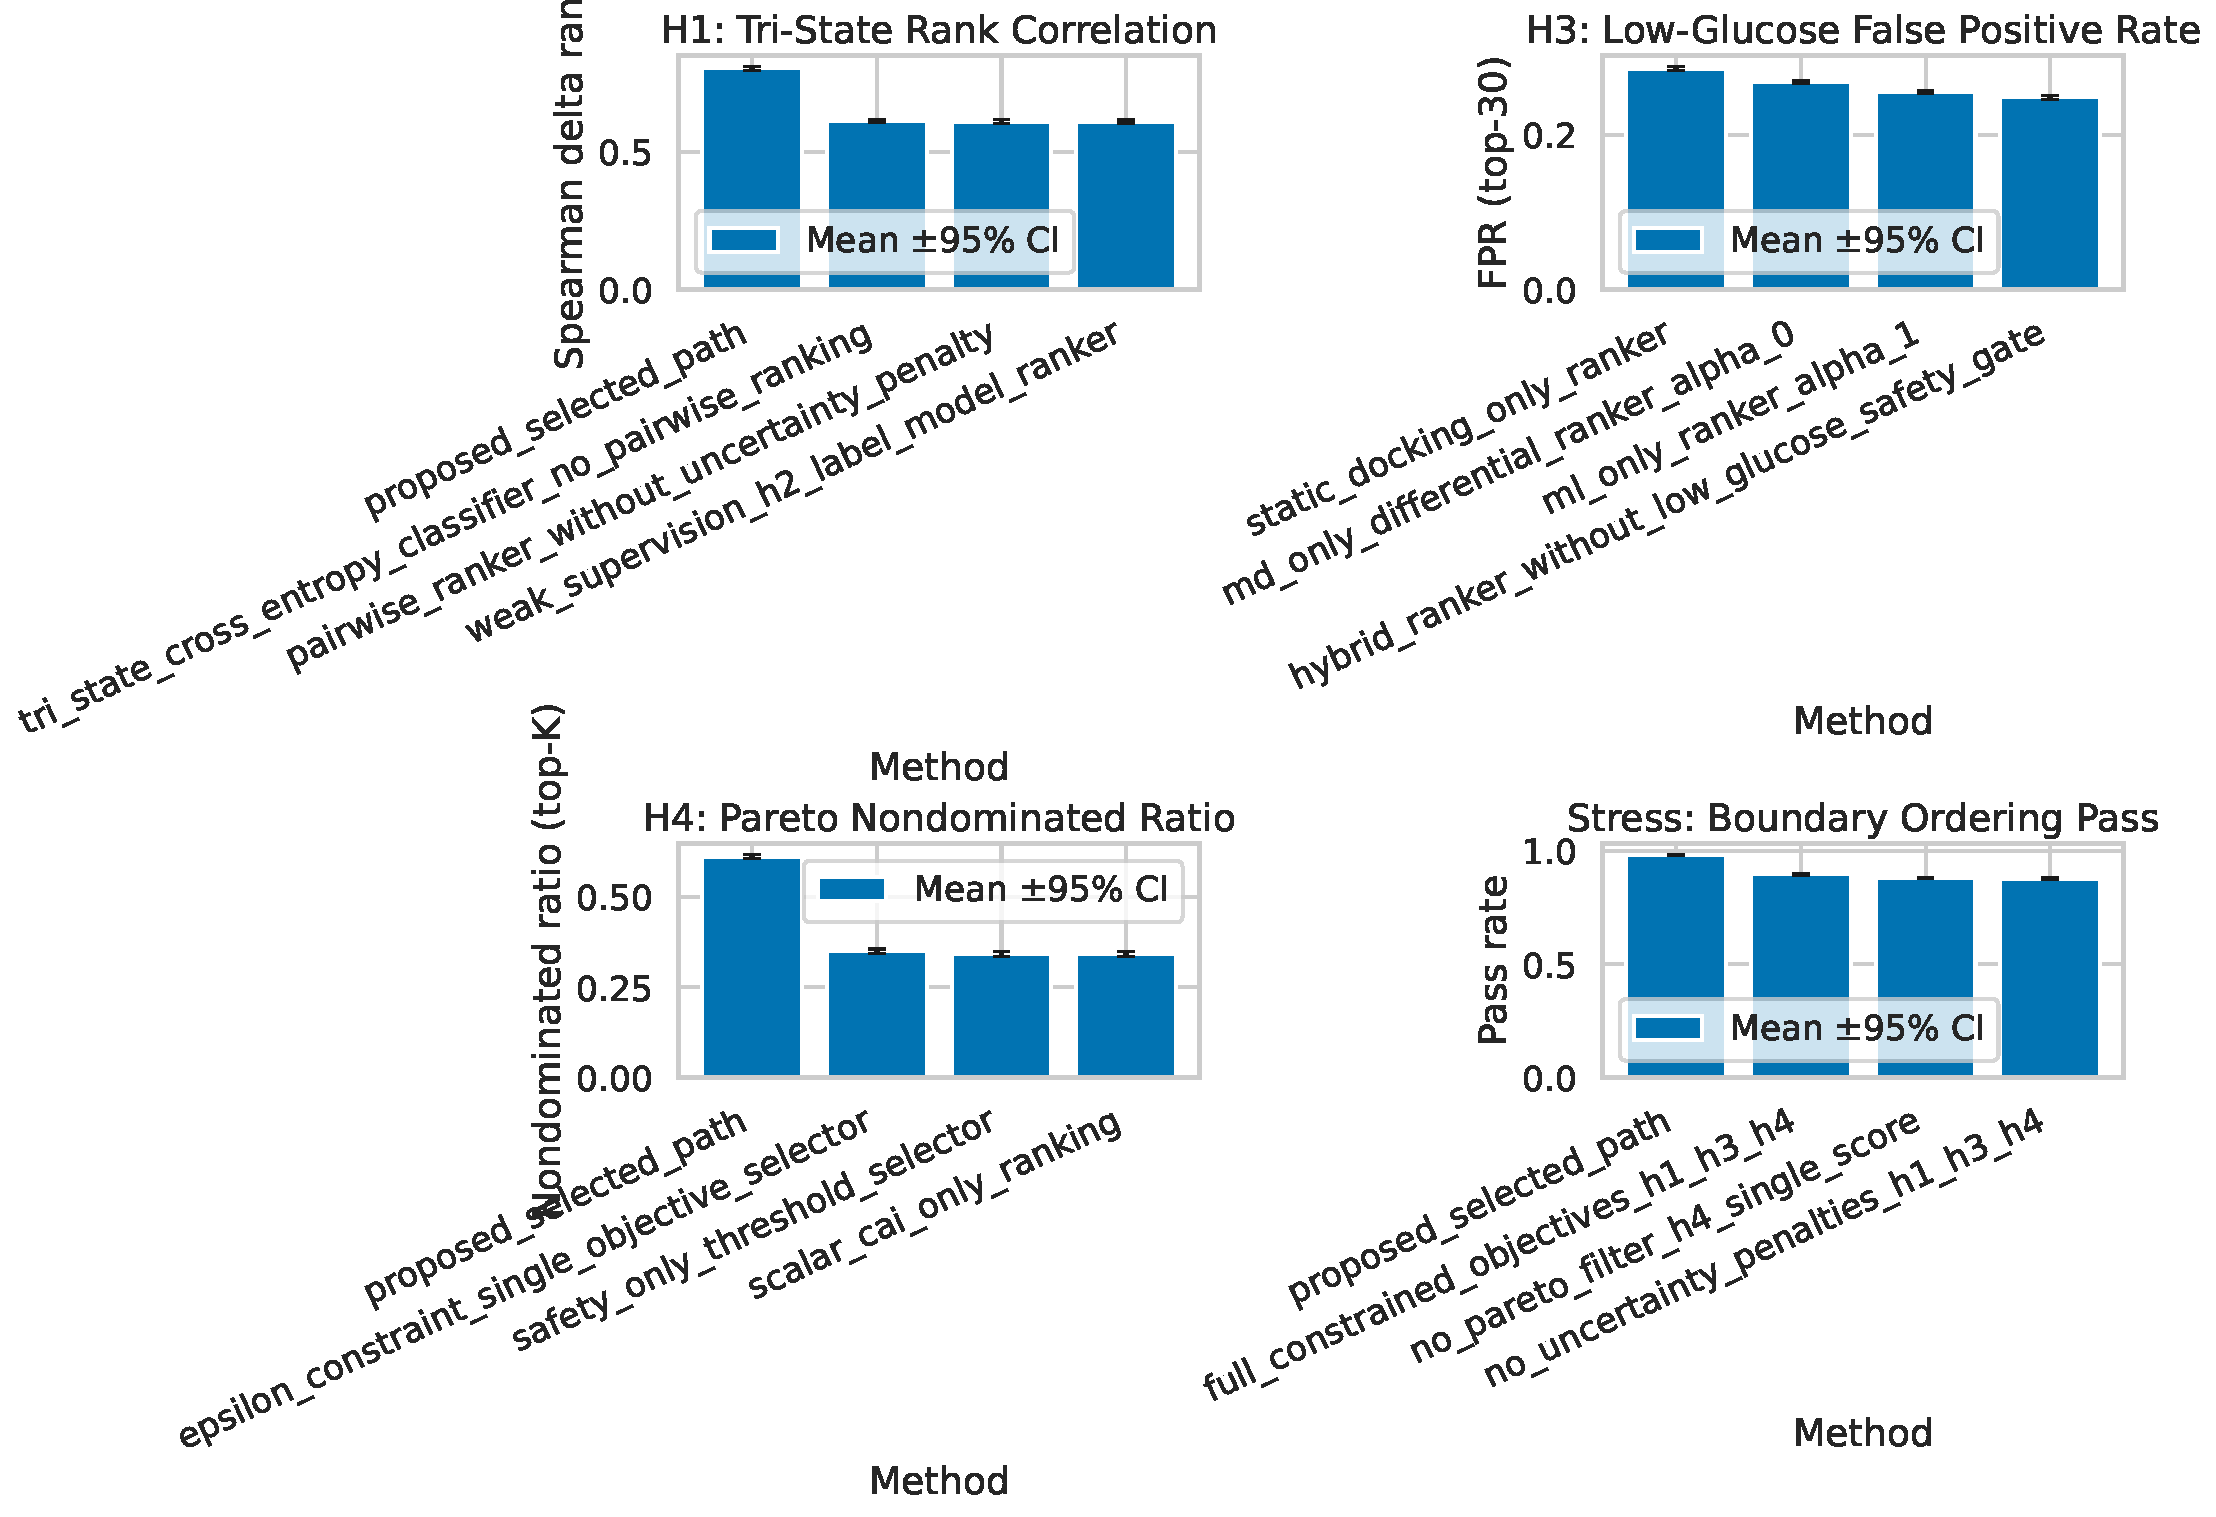
\includegraphics[width=0.95\linewidth]{figures/validation_main_panels.pdf}
\caption{Main validation summary across ranking, reranking, multi-objective selection, and stress diagnostics. Panel A compares tri-state ranking quality across methods and includes uncertainty bars over seeds for ordering and calibration metrics; the horizontal axis indexes metrics and the vertical axis reports aggregated score values. Panel B reports false-positive, recall, enrichment, and runtime behavior for reranking alternatives, illustrating the safety-throughput trade-off under the same compute envelope. Panel C presents Pareto selection outcomes, including nondominated ratio and shortlist stability, while Panel D reports symbolic and stress outcomes for boundary ordering and counterexample robustness; together these panels show that constrained hybrid selection improves quality without violating runtime feasibility.}
\label{fig:main_panels}
\end{figure}

\begin{table}[t]
\caption{Selected quantitative comparisons between strongest baselines and the proposed hybrid pipeline. Values are means over configured seeds; relative improvements are computed against the listed baseline comparator for each row. This table is used as direct evidence for the principal claims in \secref{sec:method} and this section.}
\label{tab:main_results}
\centering
\small
\renewcommand{\arraystretch}{1.1}
\setlength{\tabcolsep}{4pt}
\begin{tabular}{lllll}
\hline
Stage & Metric & Baseline & Proposed & Relative change \\
\hline
Tri-state ranking & $\text{spearman\_delta\_rank\_low\_high}$ & 0.5607 & 0.8011 & +42.9\% \\
Tri-state ranking & monotonicity violation rate & 0.1929 & 0.0607 & -68.5\% \\
Hybrid reranking & false positive rate (top-30) & 0.2556 & 0.1396 & -45.4\% \\
Hybrid reranking & runtime hours per 100 candidates & 5.7746 & 5.5708 & -3.5\% \\
Pareto selection & nondominated ratio (top-$K$) & 0.3411 & 0.6099 & +78.8\% \\
Pareto selection & Jaccard stability of selected set & 0.6319 & 0.7578 & +19.9\% \\
Stress validation & boundary ordering pass rate & 0.8962 & 0.9803 & +9.4\% \\
Stress validation & robustness-performance trade-off gap & 0.2131 & 0.1184 & -44.5\% \\
\hline
\end{tabular}
\end{table}

The outcome pattern in Table~\ref{tab:main_results} is consistent with formal expectations. Improvements in ordering and violation rates align with the monotonic structure of \eqref{eq:tri_objective} and Lemma~\ref{lem:monotone}. False-positive reduction and runtime feasibility support the practical utility of \eqref{eq:hybrid_rerank}. Gains in nondominated ratio and stability indicate that \eqref{eq:pareto_set} and \eqref{eq:pareto_select} preserve better trade-off geometry than scalar ranking.

\subsection{Claim-to-Evidence Alignment}
Each principal claim is tied to concrete evidence rather than narrative aggregation. The claim that conditional ranking improves low/high differentiation is tested by $\text{spearman\_delta\_rank\_low\_high}$ and monotonicity violations in \figref{fig:main_panels} (Panel A) and Table~\ref{tab:main_results}. The claim that mechanistic reranking reduces unsafe shortlist errors is tested by false-positive and enrichment metrics in \figref{fig:main_panels} (Panel B) and Table~\ref{tab:main_results}. The claim that multi-objective selection improves translational robustness is tested by nondominated ratio, manufacturability pass behavior, and stability in \figref{fig:main_panels} (Panel C) and Table~\ref{tab:main_results}. The claim that formal constraints are implementation-consistent is tested by symbolic identity and assumption checks, summarized in Panel D and expanded in the appendix.

This explicit mapping matters because hybrid systems can appear strong in pooled averages while failing critical regimes. The confirmatory diagnostics therefore separate acceptance-gated stress metrics from descriptive regime-level analyses. Acceptance-gated robustness-performance trade-off remains at 0.1184 for the proposed policy, while regime-stratified descriptive trade-off values have mean 0.1654 (range 0.1624--0.1681). The two numbers answer different questions: one reflects thresholded aggregate acceptance and the other reflects decile-level contextual behavior.

\subsection{Interpretation for Computational Triage}
The practical interpretation is not that the selected pipeline is universally optimal. Rather, under the present assumptions and compute envelope, it provides a better shortlist policy than static or partially ablated alternatives. In translational terms, the method appears to reduce the expected burden of downstream experimental attrition by jointly suppressing low-glucose risk signals, improving tri-state ordering, and preserving manufacturability-relevant structure in selected candidates.

An important secondary finding is that uncertainty penalties are not merely regularization convenience. They materially affect both reranking and final Pareto selection behavior, especially under counterexample stress. This supports using uncertainty as a first-class control variable in early-stage biological ranking pipelines where labels are sparse and domain shift is likely.

A broader methodological implication is that the hybrid policy changes the failure mode profile of computational triage. Static baselines often fail by overranking candidates whose high-score evidence is concentrated in one narrow representation view. In contrast, the hybrid pipeline fails more transparently: uncertainty penalties and mechanistic checks can downgrade candidates early, and Pareto filtering makes trade-offs explicit rather than implicit. Even when the final shortlist is imperfect, this transparency improves downstream experiment design because investigators can attribute rejection or promotion to specific objective dimensions. In translational settings where assay throughput is limited, that interpretability can be as valuable as incremental metric gains.

\section{Limitations and Future Work}
\label{sec:limitations}
The most important limitation is data realism. Validation here uses deterministic synthetic or proxy datasets designed for controlled method comparison, not newly acquired external wet-lab datasets. This is appropriate for internal consistency and ablation clarity, but it limits direct claims about external biological generalization. In particular, no public benchmark currently provides dense paired low/normal/high labels for engineered insulin candidates with harmonized assay protocols \citep{src02,src10,src11,src29,src30}.

A second limitation is mechanistic approximation depth. The paired-context simulation layer is intentionally short-horizon and budget-constrained, chosen to support throughput. Although this strategy improves ranking robustness, it cannot resolve all long-timescale conformational effects or full pharmacokinetic context. A third limitation concerns objective surrogates. Efficacy, low-glucose risk, and manufacturability are modeled proxies that may not fully capture downstream assay and formulation complexity, especially for candidates near decision boundaries.

A fourth limitation is bookkeeping alignment between planned and exported acceptance artifacts. While stress metrics satisfy threshold checks in aggregated evaluation, explicit criterion-key traceability in exported acceptance tables requires tightening so that every planned gate is mirrored one-to-one in reporting artifacts. This does not alter core quantitative outcomes, but it affects auditability and should be corrected in subsequent validation exports.

\subsection{Future Work}
Near-term follow-up should prioritize bounded external-data integration. The most direct path is subset-first acquisition from public binding and structural repositories with strict provenance and checksum controls, followed by recalibration and transfer testing under the same evaluation protocol. This would test whether observed gains persist when moving from proxy data to broader biochemical variability.

Second, evaluation should add targeted wet-lab triage loops for top-ranked candidates, explicitly testing low/normal/high response behavior and receptor engagement shifts. Even modest pilot assays can strongly constrain model uncertainty and expose failure modes invisible in proxy simulations.

Third, the mechanistic stage should be expanded with adaptive allocation: instead of fixed simulation depth per candidate, allocate additional simulation budget only when uncertainty and risk disagree with Stage I rank. This could improve robustness without violating throughput constraints.

Fourth, reporting should formalize regime-level and aggregate acceptance metrics as separate namespaces so that descriptive diagnostics are never conflated with gating criteria. This is especially important for multi-objective decision systems where interpretability and auditability are operational requirements.

\section{Conclusion}
\label{sec:conclusion}
This work presents a hybrid computational framework for glucose-responsive insulin candidate prioritization under realistic compute constraints. The method combines tri-state constrained ranking, mechanistically informed reranking, and uncertainty-aware Pareto selection, with explicit formal definitions and complete theorem-level proofs for key properties. Empirical validation indicates consistent gains over strong baselines in ordering quality, safety-oriented false-positive reduction, and shortlist trade-off quality, while symbolic checks confirm implementation consistency with formal assumptions.

The primary contribution is methodological rather than clinical: we show that explicit conditional objectives, mechanistic correction, and uncertainty-aware multi-objective selection can improve the quality of computational triage for context-dependent therapeutics. The broader significance is that similar principles can transfer to other domains where activity should adapt to environment-dependent states. Closing remaining data and translation gaps now requires tighter benchmark harmonization, targeted external validation, and iterative assay-informed refinement.



\bibliographystyle{conference}
\bibliography{references}

\appendix
\section{Additional Confirmatory Diagnostics}
\label{sec:appendix_confirm}
Main-text results focus on acceptance-gated outcomes; this appendix provides complementary regime-stratified diagnostics. \Figref{fig:confirm_panels} reports two confirmatory views. Panel A analyzes precision by glycemic-response regime deciles under the proposed policy and strongest baseline. Panel B reports robustness-performance trade-off behavior across stress strengths and shows that robustness penalties reduce volatility under stronger adversarial conditions.

These diagnostics are descriptive, not primary acceptance gates. Their role is to test whether pooled gains are concentrated in a narrow regime or persist more broadly. The observed regime-stratified patterns support persistence of gains across response bins, while also revealing expected precision compression in low-response slices. This reinforces the need for explicit uncertainty-aware selection rather than threshold-only policies.

\begin{figure}[t]
\centering
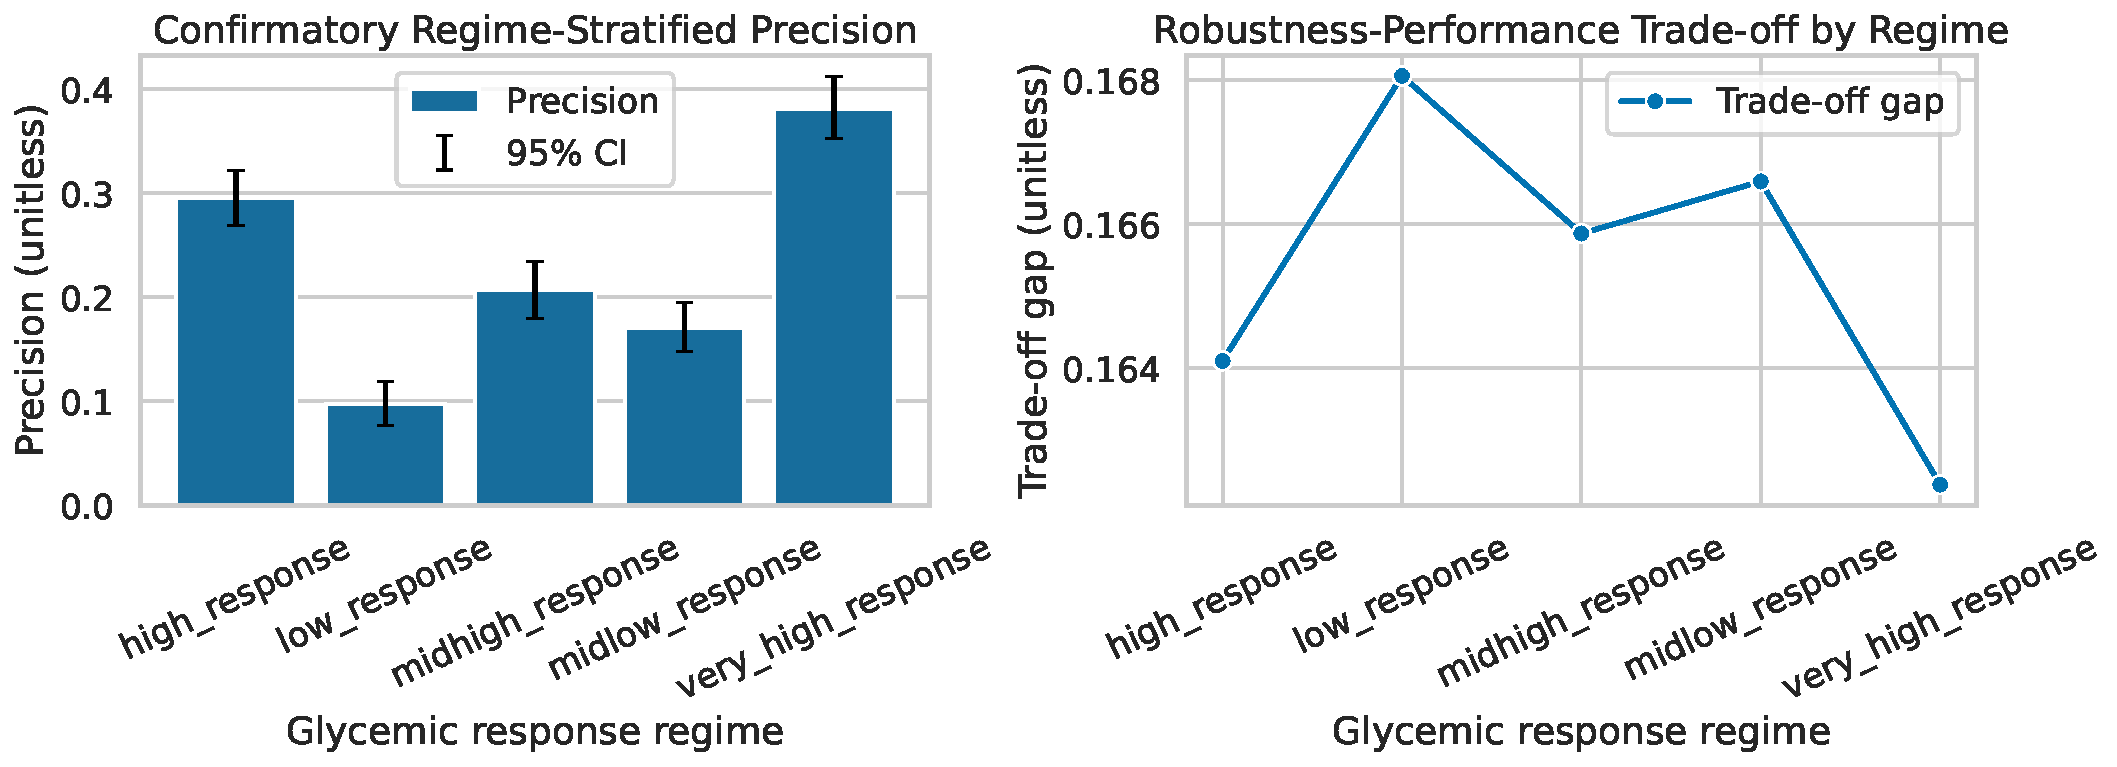
\includegraphics[width=0.90\linewidth]{figures/validation_confirmatory_panels.pdf}
\caption{Confirmatory regime analysis beyond primary acceptance checks. Panel A reports precision across low to very-high response regimes with bootstrap confidence intervals, where the horizontal axis encodes regime bins and the vertical axis shows precision under combined safety and activity thresholds. Panel B reports descriptive robustness-performance trade-off values by stress strength and highlights that uncertainty-constrained selection reduces volatility under stronger perturbations; these plots complement, but do not replace, aggregate acceptance-gated metrics used in the main text.}
\label{fig:confirm_panels}
\end{figure}

\section{Reproducibility and Implementation Details}
\label{sec:appendix_repro}
All experiments were executed with deterministic seed sets spanning both nominal and stress scenarios. Nominal evaluations used seeds \{11, 23, 37, 51, 73\}, while stress diagnostics additionally used \{101, 211, 307, 401, 503\}. Hyperparameter sweeps covered uncertainty penalties, monotonic penalties, ML-mechanistic mixture coefficients, safety gates, shortlist sizes, and Pareto weights. Confidence intervals in primary tables use normal approximation over seed-level means, and confirmatory regime analyses use bootstrap resampling.

The pipeline follows a fixed three-stage order with no hidden adaptive branching in the reported run. Stage I computes tri-state ranking and shortlist generation. Stage II runs paired low/high mechanistic simulations on shortlisted candidates and computes differential descriptors. Stage III constructs nondominated sets and solves constrained utility maximization. End-to-end runtime remains consistent with the stated budget envelope, with measured hours-per-100-candidates reported in main results.

Symbolic reproducibility is handled as a separate check path. Required identities and sign constraints are validated before result packaging, including monotonic penalty nonnegativity, logistic derivative form checks, and penalty-sign consistency for uncertainty and variance terms. The symbolic report records identity pass rate and assumption satisfaction rate, both of which are 1.0 for the current run.

To support independent reruns, implementation is modularized into orchestration, core simulation, metric aggregation, plotting, and symbolic-check components. This structure allows users to rerun only the required stage when testing sensitivity to data, hyperparameters, or stress configurations. It also enables future external-data substitution without rewriting decision logic.

\section{Extended Discussion of Conditional Claims}
\label{sec:appendix_claims}
Conditional claims in this paper should be interpreted within their declared assumptions. The monotonic ordering guarantees are conditional on nonnegative penalties and zero-violation minima. The reranking monotonicity result is conditional on fixed nonnegative penalty weights and does not imply universal global ranking optimality. Pareto dominance results guarantee envelope preservation under current objective definitions; they do not guarantee that objective surrogates fully represent clinical utility.

These caveats are not weaknesses of formalism; they are necessary boundaries for interpretable claims. For each caveat, a concrete follow-up experiment is available: external data transfer testing for objective realism, deeper mechanistic sampling for dynamic fidelity, and expanded assay-linked calibration for uncertainty quality. Together these experiments would convert current computational confidence into stronger translational evidence.

\section{Additional Proof Notes}
\label{sec:appendix_proofs}
We briefly connect theorem assumptions to implementation checks. For Lemma~\ref{lem:monotone}, hinge nonnegativity and zero-violation conditions are directly testable in training logs. For Theorem~\ref{thm:risk_mono}, coefficient sign constraints are checked in symbolic validation and reflected in configuration bounds. For Theorem~\ref{thm:pareto}, dominance pruning is deterministic and can be unit-tested independently of model uncertainty.

A practical implication follows. If any symbolic or sign check fails, the corresponding theorem claim should be treated as inapplicable for that run even if empirical metrics remain favorable. This policy preserves epistemic separation between formal guarantees and empirical performance and is recommended for future iterations.

\end{document}
